\documentclass{ximera}

% vier voorkeuren die je meteen zelf kan instellen:
\def\uitbr{0} % waarde 1 als je Uitbreiding in de marge wilt, 0 als je dat niet wilt 
\def\wsg{0} % waarde 1 als je verwijzingen naar Wiskunde Samen gevat² in de marge wilt, 0 als je dat niet wilt
\def\rectoverso{0} % waarde 1 als je het PDF-bestand recto-verso wilt laten afdrukken, 0 als je het recto wilt
\def\voetn{1} % waarde 1 als je de voetnoten wilt, 0 als je dat niet wilt 

% marges:
\usepackage[paper=a4paper,margin=3.4cm,marginparwidth=2cm]{geometry}

% packages algemeen:
\pdfOnly{
\usepackage[english,dutch]{babel}
}
\usepackage{amsfonts}
\usepackage{amsmath} %  o.a. \eqref en \text, omgeving equation*
\usepackage{amssymb} % o.a. \nmid
\usepackage{amsthm} % o.a. omgeving proof
\usepackage{graphicx} % o.a. figuren
\usepackage{xcolor} % \color
\usepackage[disable]{todonotes} % \todo 
\usepackage{comment} % omgeving comment
\usepackage{xcolor} % kleuren 
\usepackage[skip=7pt plus1pt, indent=0pt]{parskip} % skip = verticale ruimte tussen twee alinea's, indent = insprong bij nieuwe alinea
\usepackage{multicol} % kolommen
\usepackage{xfrac} % breuken

\usepackage{siunitx} % SI eenheden
\usepackage{eso-pic} % achtergrond voorpagina
\usepackage{tabularx} % kolommen voor rekenmachine
\usepackage{rotating} % voor omgeving turn

% voor figuren met PSTricks:
\usepackage{pstricks} 
\usepackage{pstricks-add}
\usepackage{pst-plot}
\usepackage{pst-node}
\usepackage{pst-coil}
\usepackage{auto-pst-pdf}

% voor figuren met TikZ:
\usepackage{tikz} 
\usepackage{tkz-euclide} 
\usepackage{pgfplots} 
\usetikzlibrary{calc,intersections,through,backgrounds,patterns} 
\pgfplotsset{compat=newest}
\usepgfplotslibrary{fillbetween,colormaps}
\usepackage{import}
\usepackage{tikz-3dplot}

% zelfde parskip in minipage:
\makeatletter
\setlength{\parskip}{\medskipamount}
\newcommand{\@minipagerestore}{\setlength{\parskip}{\medskipamount}}
\makeatother

% voor veranderen van de naam Bibliografie naar Referentielijst:
\pdfOnly{
\addto\captionsdutch{\renewcommand{\bibname}{Referentielijst}}

% voor trefwoordenlijst:
\usepackage{imakeidx}
\makeindex[title=Trefwoordenlijst,program=makeindex,options=-s index.tex,columns=2,intoc=true]
}
% voor nummeren van vergelijkingen:
%WIM%\numberwithin{equation}{chapter} % als je dit desactiveert dan worden vergelijkingen in bijvoorbeeld hoofdstuk 3 genummerd als (1), (2) etc. in plaats van (3.1), (3.2) etc.

% voor hyperlinks en bladwijzers in PDF-bestand:
%WIM%\usepackage[bookmarksopen,bookmarksopenlevel=0,hypertexnames=false,pdfa,bookmarksnumbered]{hyperref} 
%WIM%\usepackage{bookmark} 

% voor hyperlinks: 
\hypersetup{pdfborder={0 0 0}, pdfstartpage=1,linkbordercolor={1 0 0}}%pdfborder={0 0 0} is geen rand rond hyperlinks, pdfborder={1 1 1} wel

% korter commando voor displaystyle, om bijvoorbeeld breuken groter te drukken in doorlopende tekst: 
\newcommand{\D}{\displaystyle}

% (veel)gebruikte verzamelingen:
\newcommand\NN{\mathbb{N}} % verzameling van de natuurlijke getallen
\newcommand\QQ{\mathbb{Q}} % verzameling van de rationale getallen
\newcommand\RR{\mathbb{R}} % verzameling van de re\"ele getallen
\newcommand\ZZ{\mathbb{Z}} % verzameling van de gehele getallen

% (veel)gebruikte operatoren:
\def\co{\operatorname{co}} % coördinaat van een punt
\def\ggd{\operatorname{ggd}} % positieve grootste gemene deler van twee gehele getallen niet beide nul
\def\gr{\operatorname{gr}} % graad van een veelterm

% voor kleur grafieken (donkergroen):
\definecolor{graf}{RGB}{0,100,0} 

% voor lijsten: 
% \usepackage{enumerate}
%WIM%\usepackage[shortlabels]{enumitem} 
\setlist{topsep=0em, itemsep=-0.15em}

% voor small bullet:
\newcommand\sbullet[1][.5]{\mathbin{\vcenter{\hbox{\scalebox{#1}{$\bullet$}}}}}

% voor meer verticale ruimte tussen vergelijkingen in align
\addtolength{\jot}{0.1cm}

% voor meervoudige voetnoten:
\usepackage{fnpct}

% voor het onderdrukken van voetnoten als optie:
\usepackage{letltxmacro}
\LetLtxMacro\Oldfootnote\footnote
\newcommand{\EnableFootNotes}{%
  \LetLtxMacro\footnote\Oldfootnote%
}
\newcommand{\DisableFootNotes}{%
  \renewcommand{\footnote}[2][]{\relax}
}

% voor verticale lijn in de marge (uitbreiding):
\usepackage[framemethod=default]{mdframed}
\usepackage{marginnote}
\reversemarginpar
\ifthenelse{\uitbr < 1}{\definecolor{rood}{RGB}{255,255,255}}{\definecolor{rood}{RGB}{254,64,64}} %HEX: #fe4040
\mdfdefinestyle{uitbreiding}{%
    topline=false,
    rightline=false,
    bottomline=false,
    leftline=true,
    linecolor=rood,
    linewidth=5pt,
    rightmargin=0pt,
    skipabove=10pt,% ipv 3
    skipbelow=0pt,
    leftmargin=-25pt,
    innerleftmargin=20pt,
    innerrightmargin=0pt,
    innertopmargin=0pt,
    innerbottommargin=0pt%,
%	needspace=30pt %minimumhoogte vooraleer lijn wordt gesplitst
    }
\newenvironment{Uitbreiding}{
    \marginpar{
        \center
		\vspace{0.1cm}
		\vspace{7pt}
		\rotatebox{90}{\color{rood}\Large \bf Uitbreiding}
	}
    \begin{mdframed}[style=uitbreiding]
    }{\vspace{-0.05cm}
    \end{mdframed}
}


% omgevingen voor lemma, definitie, voorbeeld etc.:
\newtheoremstyle{mystyle}
    {0em} % Space above
    {0em} % Space below
    {\itshape} % Body font
    {} % Indent amount
    {\bfseries} % Theorem head font
    {.} % Punctuation after theorem head
    {.5em} % Space after theorem head
    {} % Theorem head spec (can be left empty, meaning `normal')
\theoremstyle{mystyle}
%WIM%\newtheorem{lemma}{Lemma}[chapter] % als je [chapter] desactiveert dan Voorbeeld 3 in plaats van Voorbeeld 5.3, als je [chapter] vervangt door [section] dan Voorbeeld 5.2.3 in plaats van Voorbeeld 5.3 
%\theoremstyle{definition} % als je dit activeert dan is wat in de omgeving staat niet cursief gedrukt
\newtheorem{oefening}[lemma]{Oefening}
\newtheorem{definitie}[lemma]{Definitie} 
\newtheorem{voorbeeld}[lemma]{Voorbeeld}
\newtheorem{eigenschap}[lemma]{Eigenschap} 
\newtheorem{stelling}[lemma]{Stelling} 
\newtheorem{gevolg}[lemma]{Gevolg} 
\newtheorem{afspraak}[lemma]{Afspraak} 
\newtheorem{werkwijze}[lemma]{Werkwijze}

% omgeving proof, aangepaste ruimte: 
\makeatletter
\renewenvironment{proof}[1][\proofname]{\par
  \vspace{-\topsep}% remove the space after the theorem
  \pushQED{\qed}%
  \normalfont
  \topsep0pt \partopsep0pt % no space before
  \trivlist
  \item[\hskip\labelsep
        \itshape
    #1\@addpunct{.}]\ignorespaces
}{%
  \popQED\endtrivlist\@endpefalse
  \addvspace{0pt plus 0pt} % no space after
}
\makeatother

% kaderstijlen uit SOHO Wiskunde Plantyn:
\colorlet{steunkleur}{black}
\colorlet{steunkleurlicht}{steunkleur!30!white}
\colorlet{steunkleurkader}{steunkleur!7!white}
\colorlet{steunkleurkaderlicht}{steunkleur!2!white}

\mdfdefinestyle{kaderstijl_vol_licht}
{skipabove=6pt, 
skipbelow=6pt, 
backgroundcolor=steunkleurkader,
linecolor=steunkleurlicht,
linewidth = 0.4pt, 
topline=true,
bottomline=true, 
rightline=true,
innerleftmargin=5pt,
innerrightmargin=5pt,
innertopmargin=5pt,
leftmargin=0cm,
rightmargin=0cm,
innerbottommargin=5pt,
needspace=30pt % minimumhoogte voor splitsen kader
}
\surroundwithmdframed[style=kaderstijl_vol_licht]{definitie}
\surroundwithmdframed[style=kaderstijl_vol_licht]{stelling}
\surroundwithmdframed[style=kaderstijl_vol_licht]{lemma}
\surroundwithmdframed[style=kaderstijl_vol_licht]{eigenschap}
\surroundwithmdframed[style=kaderstijl_vol_licht]{gevolg}

% voor omgevingen voor oefening en antwoord:
\newenvironment{Oefening}{%
    \begin{enumerate}[ 
    series=Oef,
    resume=Oef,
    leftmargin=1.78em,
    label={\bfseries\arabic*.},
    ref=\arabic*
    ]
    \item %
    }{%
    \end{enumerate}
}
\newenvironment{Antwoord}{%
    \begin{enumerate}[%
    series=Antw,
    resume=Antw,
    leftmargin=1.78em,
    label={\bfseries\arabic*.},
    ref=\arabic*
    ]
    \item %
    }{%
    \end{enumerate}
}

% als de omgeving Uitbreiding start met een kaderomgeving (definitie, stelling, eigenschap, lemma of gevolg) dan moet wat extra verticale ruimte voorzien worden, met het commando \uitbreidingstartmetkader:
\def\uitbreidingstartmetkader{\mbox{}\vspace{-0.205cm}}

% % voor schema van de staartdeling:
% \usepackage{stackengine}
% \setstackgap{S}{5pt}
% \stackMath\def\stackalignment{r}
% \newcommand{\myRule}[3][white]{\textcolor{#1}{\rule{#2}{#3}}}
% \let\ph\phantom % enkel voor tekst
% \newcommand{\mph}[1]{% enkel voor math mode
%     \mathcolor{white}{#1}%
% }
% \def\staartmin{\rule{0.25cm}{0.1mm}\myRule{0.3cm}{0.1mm}}
% \def\staartphmin{\myRule{0.25cm}{0.1mm}\myRule{0.3cm}{0.1mm}}
% \newcommand{\staartstreep}[1]{\rule{\widthof{$#1$}}{0.1mm}}
% \newcommand{\staartphstreep}[1]{\myRule{\widthof{$#1$}}{0.1mm}}

% voor kolommen met schema van Horner:
\newcommand{\kolbreed}{1.0cm}
\newcolumntype{H}{>{\centering\arraybackslash$} p{\kolbreed} <{$}}

% voor nieuw commando utikzdashed: onderlijn (zoals underline) maar dan met stippellijn:
\tikzset{
    cheating dash/.code args={on #1 off #2 ends #3}{%
        \csname tikz@addoption\endcsname{%
            \pgfgetpath\currentpath%
            \pgfprocessround{\currentpath}{\currentpath}%
            \csname pgf@decorate@parsesoftpath\endcsname{\currentpath}{\currentpath}%
            \pgfmathparse{max(#1-#3,0)}\let\dashphase=\pgfmathresult%
            \pgfmathparse{\csname pgf@decorate@totalpathlength\endcsname-#1+2*\dashphase}\let\rest=\pgfmathresult%
            \pgfmathparse{#1+#2}\let\onoff=\pgfmathresult%
            \pgfmathparse{max(floor(\rest/\onoff), 1)}\let\nfullonoff=\pgfmathresult%
            \pgfmathparse{max((\rest-\onoff*\nfullonoff)/\nfullonoff+#2, #2)}\let\offexpand=\pgfmathresult%
            \pgfsetdash{{#1}{\offexpand}}{\dashphase pt}}%
    },
    cheating dash per segment/.style args={on #1 off #2 ends #3}{
        /utils/exec=\csname tikz@options\endcsname,%
        decoration={show path construction,
            lineto code={\draw [cheating dash=on #1 off #2 ends #3] (\tikzinputsegmentfirst) -- (\tikzinputsegmentlast);},
            curveto code={\draw [cheating dash=on #1 off #2 ends #3] (\tikzinputsegmentfirst) .. controls (\tikzinputsegmentsupporta) and (\tikzinputsegmentsupportb) .. (\tikzinputsegmentlast);},
            closepath code={\draw [cheating dash=on #1 off #2 ends #3] (\tikzinputsegmentfirst) -- (\tikzinputsegmentlast);}
        },
        decorate,
    },
}
\newcommand{\utikzdash}[1]{%
    \tikz[baseline=(todotted.base)]{
        \node[inner sep=0pt,outer sep=1.5pt] (todotted) {#1};
        \draw[cheating dash per segment=on 2pt off 2pt ends 2pt, line width=0.4pt] (todotted.south west) -- (todotted.south east);
    }%
}%

\providecommand{\xmemph}[1]{\textit{#1}}

% voor nieuw commando underdashed: onderlijn met stippellijnen en ook het woord cursief zetten:
\newcommand{\underdashed}[1]{%
    {\em\utikzdash{\!#1\!}}%
}

% voor icoon TI-84 Plus met verwijzing naar filmpje:
\newcommand{\grmlink}{\raisebox{0cm}{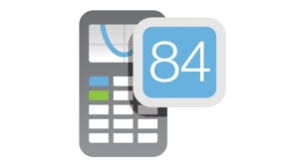
\includegraphics[width=1cm]{TI84Plus-icoon}}}
\newcommand{\grmref}[1]{%
	\reversemarginpar%
	\marginpar{
		\vspace{-0.4cm}%
		\htmladdnormallink{\grmlink}{#1}
	}	
}

% GRM knoppen:
\newcommand{\GRM}[1]{\fbox{\rule[0mm]{0cm}{0.215cm}\textup{\texttt{#1}}}}
\newcommand{\wedgetext}{{\raisebox{0.02cm}{\begin{turn}{90}>\end{turn}}}}
\newcommand{\veetext}{\raisebox{0.2cm}{\begin{turn}{-90}>\end{turn}}}

% voor kolommen met GRM screens:
\newlength{\widthallscreens}
\newlength{\widthscreens}
\newlength{\spaceleftscreen}
\newlength{\spacerightscreen}
\newlength{\spacebetweenscreens}

\newcommand{\setscreens}{
	\setlength{\spaceleftscreen}{2pt}
	\setlength{\spacerightscreen}{2pt}
	\setlength{\spacebetweenscreens}{8pt}
	\addtolength{\linewidth}{-28pt} % 3*8pt tussen vier screens en 2 pt links en 2 pt rechts
	\setlength{\widthallscreens}{\linewidth}
	\setlength{\widthscreens}{0.25\widthallscreens}
	\addtolength{\linewidth}{28pt}
	\newcolumntype{G}{p{\widthscreens}}
	\newcolumntype{s}{p{\spacebetweenscreens}}
	\newcolumntype{L}{p{\spaceleftscreen}}
	\newcolumntype{R}{p{\spacerightscreen}}
	\setlength{\tabcolsep}{0pt}
}

% voor icoon met verwijzing naar Wiskunde Samen gevat² in de marge:
% \newcommand{\wsglink}{\raisebox{0cm}{\includegraphics[width=1cm]{wsglogo}}}
\newcommand{\wsglink}{\raisebox{0cm}{LOGO}}
\newcommand{\htmladdnormallink}[2]{\href{#2}{#1}}
\newcounter{pagnrwsg}
\newcommand{\wsgref}[3]{% 
    % #1 woord dat onderstippeld wordt
    % #2 pagina van Wiskunde Samen gevat² waar je op terecht komt als je op de link klikt  
    % #3 afgedrukt op het logo van Wiskunde Samen gevat² in de marge: één of meerdere paginanummers
    \ifthenelse{\wsg < 1}{#1}{%
        \underdashed{#1}%
        {\setcounter{pagnrwsg}{#2}}%
        {\addtocounter{pagnrwsg}{14}}%
        \reversemarginpar%
        \marginpar{\vspace{-0.6cm}%
           \htmladdnormallink{\wsglink}{https://online.fliphtml5.com/sanky/laea/\#p=\arabic{pagnrwsg}}%
            \raisebox{0.41cm}[0cm][0cm]{%
                \hspace{-1.5cm}\makebox[2cm][c]{\colorbox{white}{\texttt{\footnotesize{#3}}}}%
            }%
        }%
    }%
}

% voor invoegen blanco pagina bij de optie recto-verso:
\def\blancobijrectoverso{
	\ifthenelse{\rectoverso < 1}{\clearpage}{
	\clearpage
	\thispagestyle{empty}
	\mbox{}
	\clearpage
	}
}

% aantal pagina's van het bestand:
\ifthenelse{\rectoverso < 1}{\def\totpag{57}}{\def\totpag{66}}

% documenteigenschappen:
% \usepackage{hyperxmp}
% \hypersetup{
% pdftitle={Open Source Wiskunde Aan zet: Veeltermen}, 
% pdfnumpages={\totpag},
% pdfauthor={Koen De Naeghel},
% pdflang={nl},
% pdfkeywords={wiskunde, open source, wiskunde aan zet, veeltermen, secundair onderwijs, tweede graad, doorstroomfinaliteit},
% pdfsubject={Veeltermen},
% pdfcopyright={\unichar{"24B8} 2024 Koen De Naeghel},
% pdfdate={17 december 2024},
% pdfapart=1,
% pdfstartview=}

% voor het benoemen van titel, auteur en datum:
% \title{Veeltermen}
% \author{Auteur: Koen De Naeghel}
% \date{\today}

\newcommand\BackgroundPic{
    \put(-260,-125){
    \parbox[b][\paperheight]{\paperwidth}{%
    \vfill
    \centering
    
\includegraphics[height=\paperwidth, keepaspectratio]{WaZlogo}%
    \vfill
}}}

\addPrintStyle{..}

\begin{document}
    \author{Kwinten Obbels}
    \xmtitle{Intro: nieuwe getallen voor vergelijkingen}{}

Doorheen de geschiedenis van de wiskunde hebben nieuwe getallen een belangrijke rol gespeeld.
Uit het tellen komen de meest eenvoudige getallen voort: 1 appel, 2 appels, 3 appels, ... 
Dit zijn de natuurlijke getallen, die genoteerd worden met de letter \( \N = \{0, 1, 2, 3, 4, 5, 6, ...\} \) . 

Met deze getallen kan je op verschillende manieren 'nieuwe getallen' invoeren. 
Door negatieve getallen toe te voegen wordt de verzameling getallen groter.  
Dit zijn de gehele getallen, die genoteerd worden met de letter  \( \Z = \{..., -5, -4, -3, -2, -1, 0, 1, 2, 3, 4, 5, ...\} \) . 

Wiskundigen hebben allerlei redenen om nieuwe getallen in te voeren, waaronder het oplossen van vergelijkingen. 
De vergelijking \(x + 2 = 1\) heeft bijvoorbeeld geen oplossing in de natuurlijke getallen.
Zonder het gehele getal \(x = -1\) is deze vergelijking niet oplosbaar. 


%dit moet een optionele denkvraag zijn; indien de leerkracht ze kiest staat ze erbij. 
%bij de historische inleiding zijn niet non negotiable; een leerkracht zonder denkvragen krijgt die toch als ze historische inleiding kiest 
\begin{denkvraag*}{}
    De Oude Grieken hebben negatieve getallen nooit aanvaard. 
    Voor hen is een getal altijd een hoeveelheid of een lengte, en dus positief. 
    \textbf{Ben jij akkoord met de Oude Grieken?}
    \\
\begin{tabular}{@{\qquad}l}
    Bestaan negatieve getallen wel 'écht'? \\
    Je hebt 1 appel, 2 appels, 3 appels, ... Maar wat is precies '-1 appel'? \\
    Aan welke vereisten moet iets voldoen voordat jij het 'een getal' zou willen noemen? \\
\end{tabular}
\end{denkvraag*}


Breuken leiden tot een volgende uitbreiding van de getallen.
%kunnen de gehele getallen \(\Z \) verder uitgebreid worden. 
Die nieuwe getallen worden de rationale getallen genoemd, en genoteerd met de letter \( \Q  = \left\{ \frac{z}{n} \mid z \in \Z, n \in \Nnul \right\}\).
Voorbeelden zijn \(\frac{2}{3}\), \(\frac{-4}{3}\), \(\frac{1}{1}\) en \(\frac{0}{3}\). 
Ook rationale getallen zijn nuttig om vergelijkingen op te lossen, 
want de vergelijking \(3x + 4 = 0\) heeft geen oplossing in de gehele getallen \( \Z \).
Zonder de breuk \(x = \frac{-4}{3}\) is deze vergelijking niet oplosbaar.

Je merkt al snel dat je nog niet 'genoeg' getallen hebt. 
De stelling van Pythagoras 
leert ons dat de schuine zijde van onderstaande driehoek lengte \( \sqrt{2}\) heeft. 


\begin{image}[3cm]
    
    \begin{tikzpicture}[scale=2]
        % Define the vertices of the triangle
        \coordinate (A) at (0,0);
        \coordinate (B) at (1,0);
        \coordinate (C) at (0,1);
        % Draw the triangle
        \draw (A) -- (B) -- (C) -- cycle;
        
        % Label the hypotenuse with sqrt(2)
        \node at ($(B)!0.5!(C)$) [above right] {$\sqrt{2}$};
        \node at ($(A)!0.5!(B)$) [below] {$1$};
        \node at ($(A)!0.5!(C)$) [left] {$1$};
        
    \end{tikzpicture}
\end{image}
    
Met een kort bewijs kan men aantonen dat \(\sqrt{2}\) niet in de verzameling rationale getallen zit, dus dat 
\[\sqrt{2} = 1.4142135623730950488016887242096980785696718753769480731766797\ldots%379907324784621070388503875343276...
\]  
niet te schrijven is als een breuk!. 
Deze getallen worden \textit{irrationaal} genoemd en hebben altijd oneindig veel cijfers na de komma.
%
Andere voorbeelden zijn 
\[ \pi = 3.141592653589793238462643383279502884197169399375\ldots%105820974944592307816406286208998628034825342117... 
,
\frac{\sqrt{2}}{2}
\Ten \pi^2 
\]
%
Ook irrationale getallen zijn nuttig om vergelijkingen op te lossen. 
De vergelijking \(x^2 + 2 = 4\) heeft immers geen oplossing in de rationale getallen \( \Q \).
Zonder het irrationale getal \(x = \sqrt{2} \) kan je deze vergelijking niet oplossen.
Als de irrationale getallen worden toegevoegd aan de rationale getallen \(\Q\), bekom je de reële getallen \(\R\). 
De reële getallen vormen een rechte waarbij met elk punt een reëel getal overeenkomt. 


% \begin{image}[0.7\textwidth]
%     % BRON: Ingmar !

%     \tikzset{every picture/.style={line width=0.75pt}} %set default line width to 0.75pt        
    
%     \begin{tikzpicture}[x=0.75pt,y=0.75pt,yscale=-1,xscale=1]
%     %uncomment if require: \path (0,172); %set diagram left start at 0, and has height of 172
    
%     %Shape: Ellipse [id:dp7922358117606259] 
%     \draw  [draw opacity=1 ] (230,92) .. controls (230,71.57) and (266.04,55) .. (310.5,55) .. controls (354.96,55) and (391,71.57) .. (391,92) .. controls (391,112.43) and (354.96,129) .. (310.5,129) .. controls (266.04,129) and (230,112.43) .. (230,92) -- cycle ;
%     %Shape: Ellipse [id:dp27778820345068733] 
%     \draw  [draw opacity=1 ] (163,91.5) .. controls (163,66.37) and (218.52,46) .. (287,46) .. controls (355.48,46) and (411,66.37) .. (411,91.5) .. controls (411,116.63) and (355.48,137) .. (287,137) .. controls (218.52,137) and (163,116.63) .. (163,91.5) -- cycle ;
%     %Shape: Ellipse [id:dp2930830644400444] 
%     \draw  [draw opacity=1 ] (103,92.5) .. controls (103,60.74) and (175.31,35) .. (264.5,35) .. controls (353.69,35) and (426,60.74) .. (426,92.5) .. controls (426,124.26) and (353.69,150) .. (264.5,150) .. controls (175.31,150) and (103,124.26) .. (103,92.5) -- cycle ;
%     %Shape: Ellipse [id:dp715353025232164] 
%     \draw  [draw opacity=1 ] (28,91.5) .. controls (28,54.77) and (119.56,25) .. (232.5,25) .. controls (345.44,25) and (437,54.77) .. (437,91.5) .. controls (437,128.23) and (345.44,158) .. (232.5,158) .. controls (119.56,158) and (28,128.23) .. (28,91.5) -- cycle ;
    
%     % Text Node
%     \draw (292,74.4) node [anchor=north west][inner sep=0.75pt]  [font=\LARGE]  {$\mathbb{N}$};
%     \draw (195,75.4) node [anchor=north west][inner sep=0.75pt]  [font=\LARGE]  {$\mathbb{Z}$};
%     \draw (125,74.4) node [anchor=north west][inner sep=0.75pt]  [font=\LARGE]  {$\mathbb{Q}$};
%     \draw ( 62,76.4) node [anchor=north west][inner sep=0.75pt]  [font=\LARGE]  {$\mathbb{R}$};    
    
%     \end{tikzpicture}
% \end{image}    



In het vierde jaar heb je geleerd hoe je de tweedegraadsvergelijking \(ax^2 + bx + c = 0\) kan oplossen. 
Hierbij maakte je een onderscheid naargelang het teken van de discriminant \(D = b^2 - 4ac\).
De vergelijking \(x^2 + 2x + 5 = 0\) heeft als discriminant \(D = b^2 - 4ac = 4 - 20 = -16\). 
De discriminant is negatief en deze vergelijking heeft dus geen oplossingen. 
De grafiek van deze functie heeft geen snijpunten met de x-as. 

\begin{image}     
    \begin{tikzpicture}
        \begin{axis}[
            axis lines=middle,
            xlabel={$x$},
            ylabel={$y$},
            xmin=-3, xmax=1,
            ymin=0, ymax=9,
            ticks=both,
            grid=major,
            grid style={dotted, gray},
            enlargelimits=true,
            every axis x label/.style={at={(current axis.right of origin)}, anchor=north west},
            every axis y label/.style={at={(current axis.above origin)}, anchor=south east}
            ]
            % Plot the parabola
            \addplot[blue, thick, domain=-3:1, samples=100] {x^2 + 2*x + 5};
            % Add a node for the vertex
            \draw (-3, 4) node [anchor=north west][inner sep=0.75pt]  [font=\small]  {$y=x^2+2x+5$};

        \end{axis}
    \end{tikzpicture}
\end{image}
    
    
    





Je hebt geleerd dat de algemene oplossingen voor een tweedegraadsvergelijking gegeven wordt door 
\[  
    x_{1} = \frac{-b + \sqrt{D}}{2a} \quad \text{en} \quad
    x_{2} = \frac{-b - \sqrt{D}}{2a}
\]

Misschien is de formule toch zinvol? Rekenen met de negatieve discriminant geeft:

\[ x_{1,2} = \frac{-2 +- \sqrt{-16}}{2} = \frac{-2 +- 4\sqrt{-1}}{2} = -1 +- 2\sqrt{-1}\]. 

In deze 'mogelijke oplossing' staat \(\sqrt{-1}\). Omdat er geen reëel getal is met als vierkantswortel -1, heeft deze vergelijking geen oplossing in de reële getallen \(\R\). Wanneer er voor een vergelijking geen oplossing was, werden hierboven steeds nieuwe getallen toegevoegd. In dit hoofdstuk worden de reële getallen \(\R\) verder uitgebreid tot de complexe getallen \(\C\) door een nieuw getal \(i\) toe te voegen met als eigenschap dat \(i^2 = -1\). De tweedegraadsvergelijking \(x^2 + 2x + 5 = 0\) heeft dan wel oplossingen in de complexe getallen: \(-1 + 2i\)  en  \(-1-2i\).

Vandaag worden deze nieuwe 'complexe' getallen gebruikt bij het programmeren van computergames, bij het berekenen van elektronische schakelingen en in de kwantummechanica.

\begin{image}[0.7\textwidth]
    % BRON: Ingmar !

    \tikzset{every picture/.style={line width=0.75pt}} %set default line width to 0.75pt        
    
    \begin{tikzpicture}[x=0.75pt,y=0.75pt,yscale=-1,xscale=1]
    %uncomment if require: \path (0,172); %set diagram left start at 0, and has height of 172
    
    %Shape: Ellipse [id:dp7922358117606259] 
    \draw  [draw opacity=1 ] (230,92) .. controls (230,71.57) and (266.04,55) .. (310.5,55) .. controls (354.96,55) and (391,71.57) .. (391,92) .. controls (391,112.43) and (354.96,129) .. (310.5,129) .. controls (266.04,129) and (230,112.43) .. (230,92) -- cycle ;
    %Shape: Ellipse [id:dp27778820345068733] 
    \draw  [draw opacity=1 ] (163,91.5) .. controls (163,66.37) and (218.52,46) .. (287,46) .. controls (355.48,46) and (411,66.37) .. (411,91.5) .. controls (411,116.63) and (355.48,137) .. (287,137) .. controls (218.52,137) and (163,116.63) .. (163,91.5) -- cycle ;
    %Shape: Ellipse [id:dp2930830644400444] 
    \draw  [draw opacity=1 ] (103,92.5) .. controls (103,60.74) and (175.31,35) .. (264.5,35) .. controls (353.69,35) and (426,60.74) .. (426,92.5) .. controls (426,124.26) and (353.69,150) .. (264.5,150) .. controls (175.31,150) and (103,124.26) .. (103,92.5) -- cycle ;
    %Shape: Ellipse [id:dp715353025232164] 
    \draw  [draw opacity=1 ] (28,91.5) .. controls (28,54.77) and (119.56,25) .. (232.5,25) .. controls (345.44,25) and (437,54.77) .. (437,91.5) .. controls (437,128.23) and (345.44,158) .. (232.5,158) .. controls (119.56,158) and (28,128.23) .. (28,91.5) -- cycle ;
    %Rounded Rect [id:dp4008700042872797] 
    \draw  [draw opacity=1 ][line width=2.25]  (21,44.7) .. controls (21,27.47) and (34.97,13.5) .. (52.2,13.5) -- (503.8,13.5) .. controls (521.03,13.5) and (535,27.47) .. (535,44.7) -- (535,138.3) .. controls (535,155.53) and (521.03,169.5) .. (503.8,169.5) -- (52.2,169.5) .. controls (34.97,169.5) and (21,155.53) .. (21,138.3) -- cycle ;
    
    % Text Node
    \draw (292,74.4) node [anchor=north west][inner sep=0.75pt]  [font=\LARGE]  {$\mathbb{N}$};
    \draw (195,75.4) node [anchor=north west][inner sep=0.75pt]  [font=\LARGE]  {$\mathbb{Z}$};
    \draw (125,74.4) node [anchor=north west][inner sep=0.75pt]  [font=\LARGE]  {$\mathbb{Q}$};
    \draw ( 62,76.4) node [anchor=north west][inner sep=0.75pt]  [font=\LARGE]  {$\mathbb{R}$};
    \draw (487,32.4) node [anchor=north west][inner sep=0.75pt]  [font=\LARGE]  {$\mathbb{C}$};
    
    
    \end{tikzpicture}
\end{image}  


\end{document}